\section{Архитектура задачника Unix Taskbook}

%---------------------------------------------------------
%Changing visivility of the text
\begin{frame}
\frametitle{Архитектура задачника Unix Taskbook}


\begin{figure}[htbp]%
    \centering
    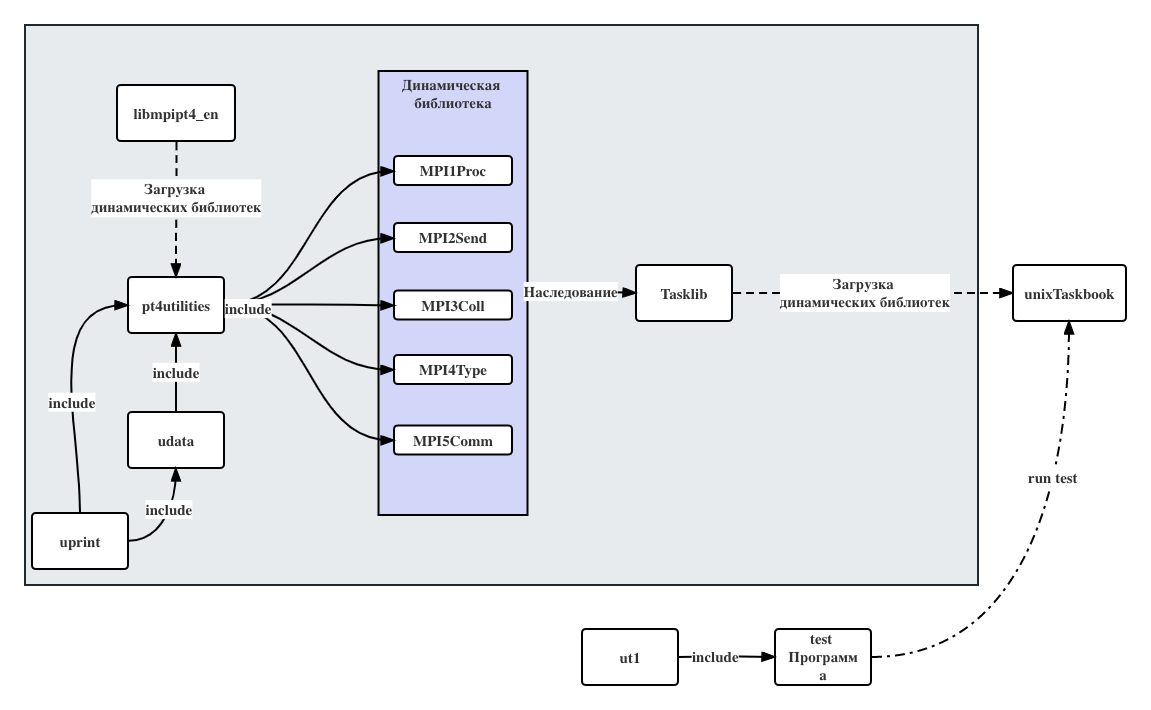
\includegraphics[width=0.8\linewidth]{images/arc.png}%子图文件名
    \caption{Отношения между динамическими библиотеками и компонентами.}%总标题
    \label{relation}%总标签
\end{figure}

% \begin{itemize}
%     \item<1-> Text visible on slide 1
%     \item<2-> Text visible on slide 2
%     \item<3> Text visible on slides 3
%     \item<4-> Text visible on slide 4
% \end{itemize}
\end{frame}

%---------------------------------------------------------


%---------------------------------------------------------
%Example of the \pause command
\begin{frame}
\frametitle{Архитектура Programming Taskbook и Unix Taskbook}
\begin{itemize}
    \item Основана на принципах, описанных в работе \cite{ref3}
    \item Включает \textbf{ядро}, обеспечивающее основную функциональность задачника, и расширяемый набор \textbf{динамических библиотек}, 
    каждая из которых содержит набор задач по определенной теме.
\end{itemize}

\end{frame}
%---------------------------------------------------------

%---------------------------------------------------------
%Example of the \pause command
\begin{frame}
\frametitle{Взаимодействие ядра и динамических библиотек}
\begin{itemize}
    \item Каждая динамическая библиотека содержит набор функций, которые вызываются из ядра на различных этапах выполнения задания:
    \begin{itemize}
        \item \textbf{этап инициализации}: генерация тестовых наборов исходных данных.
        \item \textbf{этап проверки}: сравнение полученных результатов с контрольными данными
    \end{itemize}
    \item Кроме того, в динамической библиотеке определяется \textbf{способ отображения} на экране всей информации, связанной с заданием
\end{itemize}

\end{frame}
%---------------------------------------------------------